%%%%%%%%%%%%%%%%%%%%%%%%%%%%%%%%%%%%%%%%%
% baposter Portrait Poster
% LaTeX Template
% Version 1.0 (15/5/13)
%
% Created by:
% Brian Amberg (baposter@brian-amberg.de)
%
% This template has been downloaded from:
% http://www.LaTeXTemplates.com
%
% License:
% CC BY-NC-SA 3.0 (http://creativecommons.org/licenses/by-nc-sa/3.0/)
%
%%%%%%%%%%%%%%%%%%%%%%%%%%%%%%%%%%%%%%%%%

%----------------------------------------------------------------------------------------
%	PACKAGES AND OTHER DOCUMENT CONFIGURATIONS
%----------------------------------------------------------------------------------------

\documentclass[a0paper,portrait]{baposter}

%841mm x 1189mm
\usepackage[font=small,labelfont=bf]{caption} % Required for specifying captions to tables and figures
\usepackage{booktabs} % Horizontal rules in tables
\usepackage{relsize} % Used for making text smaller in some places
\usepackage[urlcolor  = blue]{hyperref}
\graphicspath{{figures/}} % Directory in which figures are stored

\usepackage[spanish]{babel}

\usepackage[utf8]{inputenc}
\usepackage[T1]{fontenc}
\usepackage{lmodern}
\usepackage{graphicx}
\usepackage{amsmath, amssymb, bm}
\usepackage{booktabs}
\usepackage{qrcode}
\usepackage{physics}
\usepackage{tikz}
\usepackage{geometry}
\usepackage{hyperref}
\geometry{margin=1cm}

\usepackage{qrcode}
\usetikzlibrary{arrows.meta, positioning, shapes.geometric}

% \definecolor{bordercol}{RGB}{5,2,82} % Border color of content boxes
% \definecolor{headercol1}{RGB}{5,2,82} % Background color for the header in the content boxes (left side)
% \definecolor{headercol2}{RGB}{5,2,82} % Background color for the header in the content boxes (right side)
% \definecolor{headerfontcol}{RGB}{255,255,255} % Text color for the header text in the content boxes
% \definecolor{boxcolor}{RGB}{255,255,255} % Background color for the content in the content boxes

% % --- Paleta 1: Moderno y Profesional ---
% \definecolor{bordercol}{RGB}{46,86,120}      % Borde: Un azul acero oscuro
% \definecolor{headercol1}{RGB}{70,130,180}     % Header: Azul acero principal
% \definecolor{headercol2}{RGB}{70,130,180}     % Header: Mismo azul para un look uniforme
% \definecolor{headerfontcol}{RGB}{255,255,255} % Texto del Header: Blanco puro para contraste
% \definecolor{boxcolor}{RGB}{245,248,250}      % Fondo de la caja: Un gris muy claro para reducir el brillo

% --- Paleta 2: Académico y Natural ---
\definecolor{bordercol}{RGB}{0,77,75}         % Borde: Verde azulado muy oscuro
\definecolor{headercol1}{RGB}{0,107,104}       % Header: Verde azulado (teal) principal
\definecolor{headercol2}{RGB}{0,107,104}       % Header: Mismo verde
\definecolor{headerfontcol}{RGB}{255,255,255} % Texto del Header: Blanco
\definecolor{boxcolor}{RGB}{250,249,246}      % Fondo de la caja: Un blanco arena muy sutil

% % --- Paleta 3: Cálido y Energético ---
% \definecolor{bordercol}{RGB}{54,69,79}        % Borde: Gris carbón oscuro
% \definecolor{headercol1}{RGB}{199,93,40}       % Header: Terracota o naranja quemado
% \definecolor{headercol2}{RGB}{199,93,40}       % Header: Mismo terracota
% \definecolor{headerfontcol}{RGB}{255,255,255} % Texto del Header: Blanco
% \definecolor{boxcolor}{RGB}{248,248,248}      % Fondo de la caja: Blanco con un ligero toque gris



\usetikzlibrary{shapes.geometric, arrows.meta, positioning}

\definecolor{tikzHeaderGreen}{RGB}{0,107,104}   % Verde principal
\definecolor{tikzProcessSand}{RGB}{210,140,60}  % Un tono arena/ocre para contraste
\definecolor{tikzDecisionRust}{RGB}{190,80,70}   % Un rojo terroso/óxido para las decisiones

\tikzset{
    % Estilos con colores de la Paleta 2
    startstop/.style={
        rectangle, rounded corners, minimum width=3.5cm, minimum height=1cm, 
        text centered, very thick,
        draw=tikzHeaderGreen!80!black, % Borde verde oscuro
        fill=tikzHeaderGreen!15         % Relleno verde muy claro
    },
    process/.style={
        rectangle, minimum width=3.5cm, minimum height=1cm, text centered, very thick,
        draw=tikzProcessSand!80!black,  % Borde ocre oscuro
        fill=tikzProcessSand!15         % Relleno ocre muy claro
    },
    decision/.style={
        diamond, aspect=2, text centered, very thick,
        draw=tikzDecisionRust!80!black, % Borde rojo óxido oscuro
        fill=tikzDecisionRust!20        % Relleno rojo óxido claro
    },
    arrow/.style={thick, ->, >=Stealth}
}
% \tikzset{
%     % Estilos básicos
%     startstop/.style={rectangle, rounded corners, minimum width=3.5cm, minimum height=1cm, text centered, draw=blue!80!black, fill=blue!10, very thick},
%     process/.style={rectangle, minimum width=3.5cm, minimum height=1cm, text centered, draw=purple!80!black, fill=purple!10, very thick},
%     decision/.style={diamond, aspect=2, text centered, draw=red!80!black, fill=red!10, very thick},
%     arrow/.style={thick, ->, >=Stealth}
% }


\begin{document}

\background{ % Set the background to an image (background.pdf)

}

\begin{poster}{
colspacing=0.5em,
grid=false,
borderColor=bordercol, % Border color of content boxes
headerColorOne=headercol1, % Background color for the header in the content boxes (left side)
headerColorTwo=headercol1, % Background color for the header in the content boxes (right side)
headerFontColor=headerfontcol, % Text color for the header text in the content boxes
boxColorOne=boxcolor, % Background color for the content in the content boxes
headershape=roundedright, % Specify the rounded corner in the content box headers
headerfont=\large\sf\bf, % Font modifiers for the text in the content box headers
textborder=rectangle,
background=user,
headerborder=open, % Change to closed for a line under the content box headers
boxshade=plain
}
{}
%
%----------------------------------------------------------------------------------------
%	TITLE AND AUTHOR NAME
%----------------------------------------------------------------------------------------
%
%\vspace{2em}
{
%\newline
\Large\sf\bf Explorando Sistemas Cuánticos con Python: Una guía para el salón de clases.} % Poster title
{Rafael Corella, Bryan Campa, Carlos Felix, Dr. Adrian Duarte\\ % Author names
%\vspace{1em}
Universidad de Sonora
%\vspace{1em}
} % Author email addresses
%

%----------------------------------------------------------------------------------------
%	INTRODUCTION
%----------------------------------------------------------------------------------------

\headerbox{Enfoque Pedagógico}{name=ped,column=2,row=0,span=1}{
  El proyecto promueve el aprendizaje progresivo según la taxonomía de Bloom; desde comprender, hasta llegar a evaluar y crear.

  A través del desarrollo de código, el estudiante transita desde la comprensión de la ecuación de Schrödinger hasta la creación de modelos autoconsistentes.
}


\headerbox{Introducción}{name=intro,column=0,row=0, span=2,bottomaligned=ped}{
Se desarrollaron implementaciones desde cero de los métodos computacionales fundamentales en la física cuántica: el método de \textbf{Numerov} y el método de \textbf{Hartree-Fock}.

El propósito de este trabajo no es solo resolver sistemas cuánticos simples, sino fomentar un pensamiento de orden superior mediante la construcción explícita de los algoritmos que subyacen a la teoría.

El estudio detallado de estos métodos permite al estudiante conectar la formulación matemática con su representación numérica, desarrollando intuición física y criterio computacional.
}
%--------------------------------------------------
%	Hartree-Fock
%--------------------------------------------------

\headerbox{Método de Hartree–Fock}{name=hf,column=0,below=intro,span=2}{
  El método de Hartree–Fock aproxima el estado fundamental de un sistema de $N$ electrones mediante un determinante de Slater que minimiza la energía total bajo el principio variacional.  
  Este procedimiento conduce a las ecuaciones de Roothaan–Hall, resueltas iterativamente en un ciclo de campo medio (SCF):

  \begin{equation}
  \label{eq:1}
  \mathbf{F}\mathbf{C} = \mathbf{S}\mathbf{C}\boldsymbol{\varepsilon}
  \end{equation}

  donde $\mathbf{F}$ es la matriz de Fock, $\mathbf{S}$ la de solapamiento, $\mathbf{C}$ los coeficientes moleculares y $\boldsymbol{\varepsilon}$ los valores propios orbitales.

  \begin{itemize}
    \item Proporciona las energías y los orbitales moleculares en el marco del campo medio.  
    \item La densidad electrónica $\rho(\mathbf{r})$ describe la distribución espacial de carga en el sistema.  
    \item Constituye la base para métodos de correlación electrónica y DFT.
  \end{itemize}

  \begin{center}
  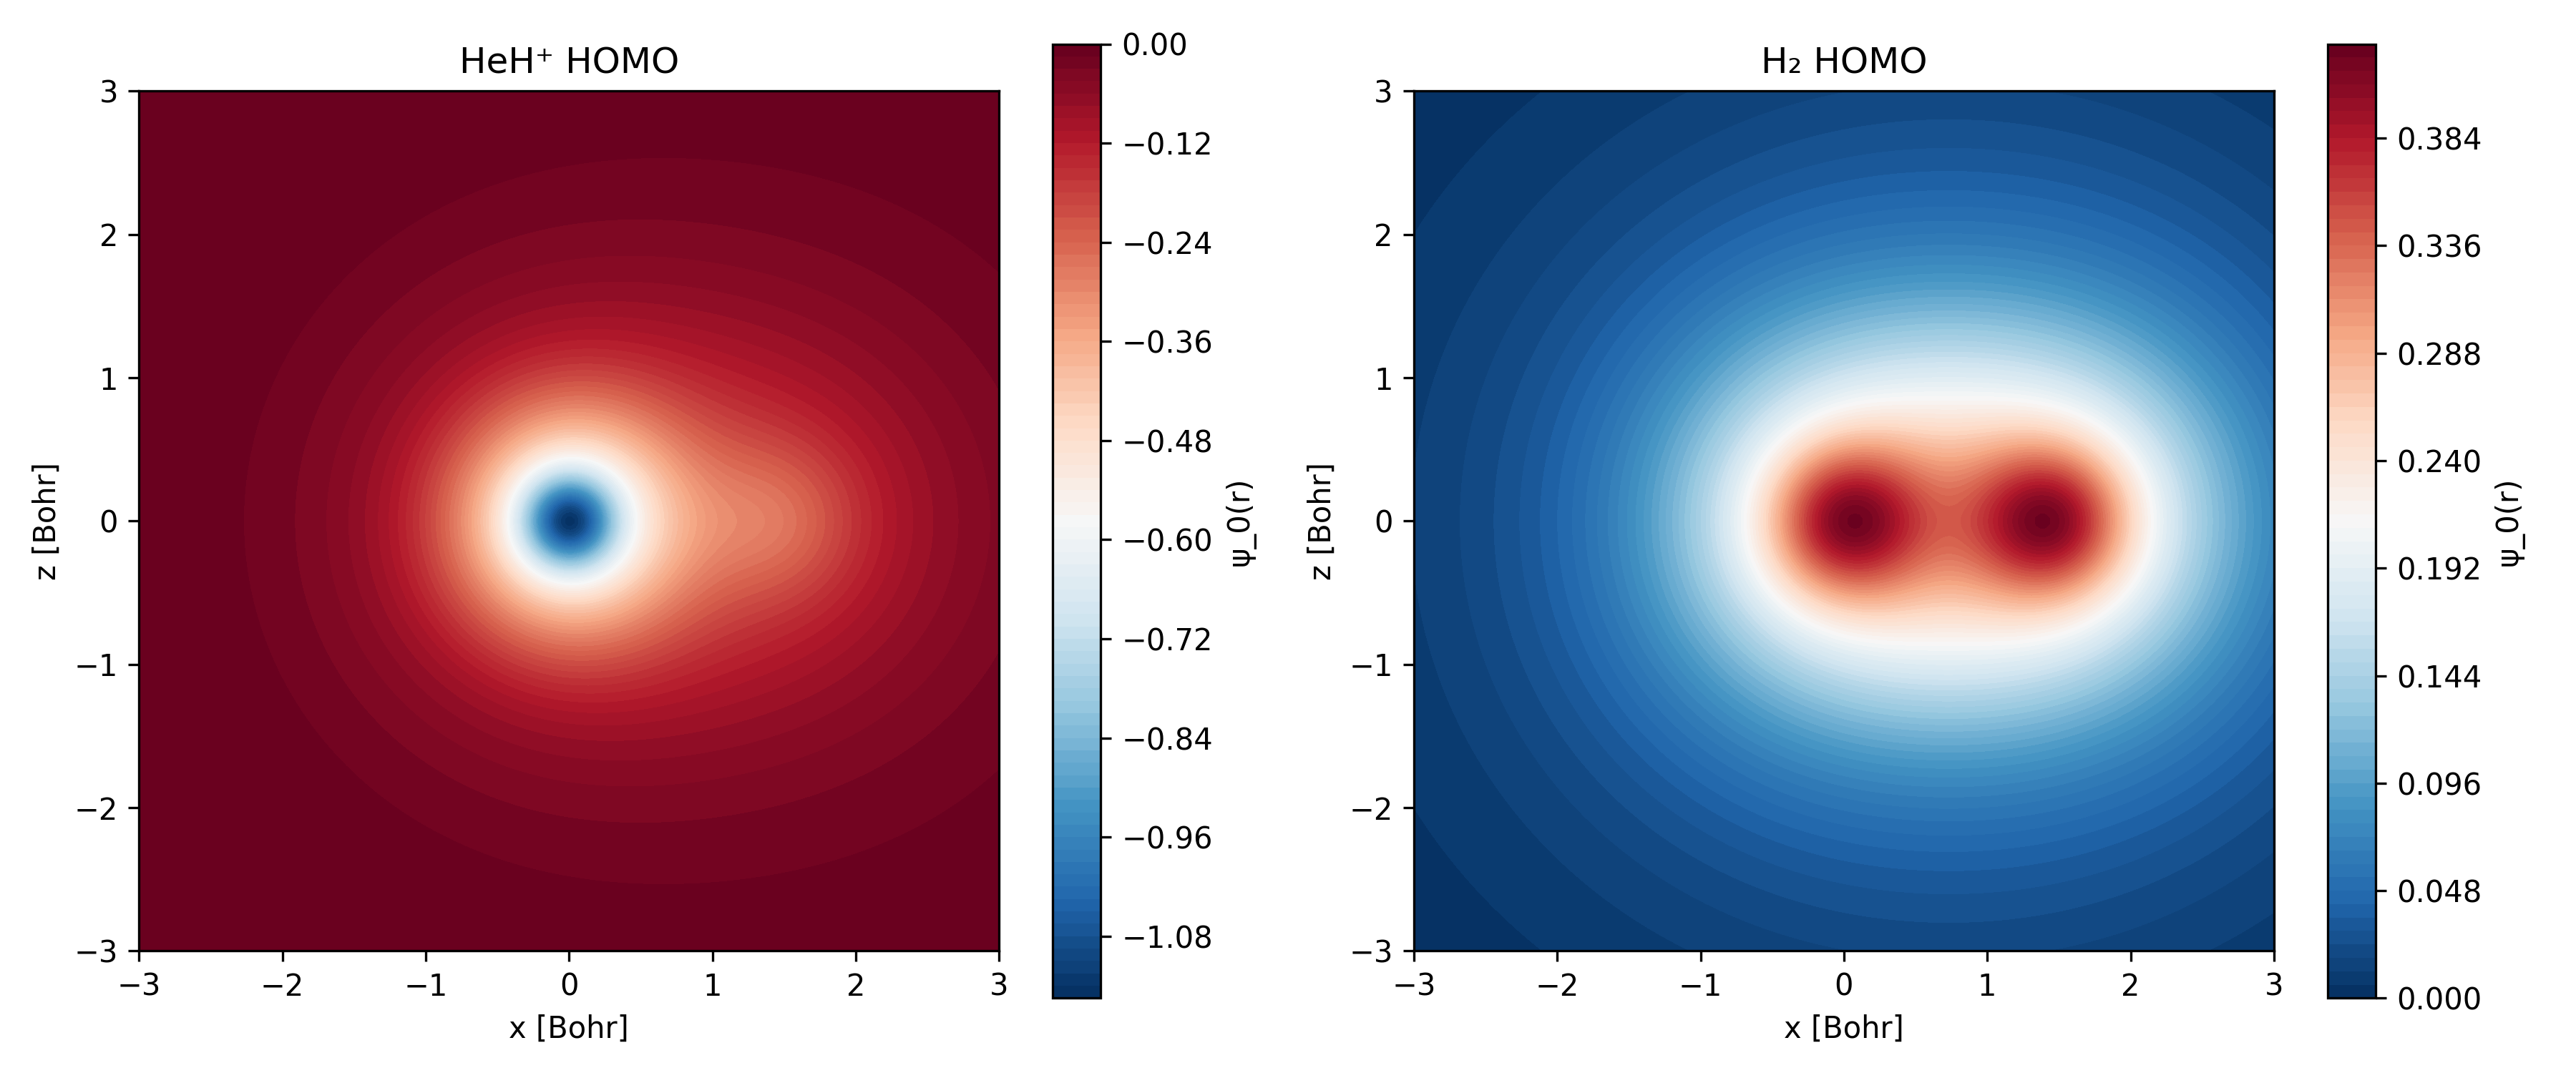
\includegraphics[width=0.9\linewidth]{molecular_orbitals.png}
  \captionof{figure}{Rebanada $xz$ de Orbitales Moleculares para H$_2$ y HeH$^+$.}
  \end{center}
}
\headerbox{Átomo de Hidrógeno}{name=code1,column=1,below=hf,span=1}{

\begin{center}
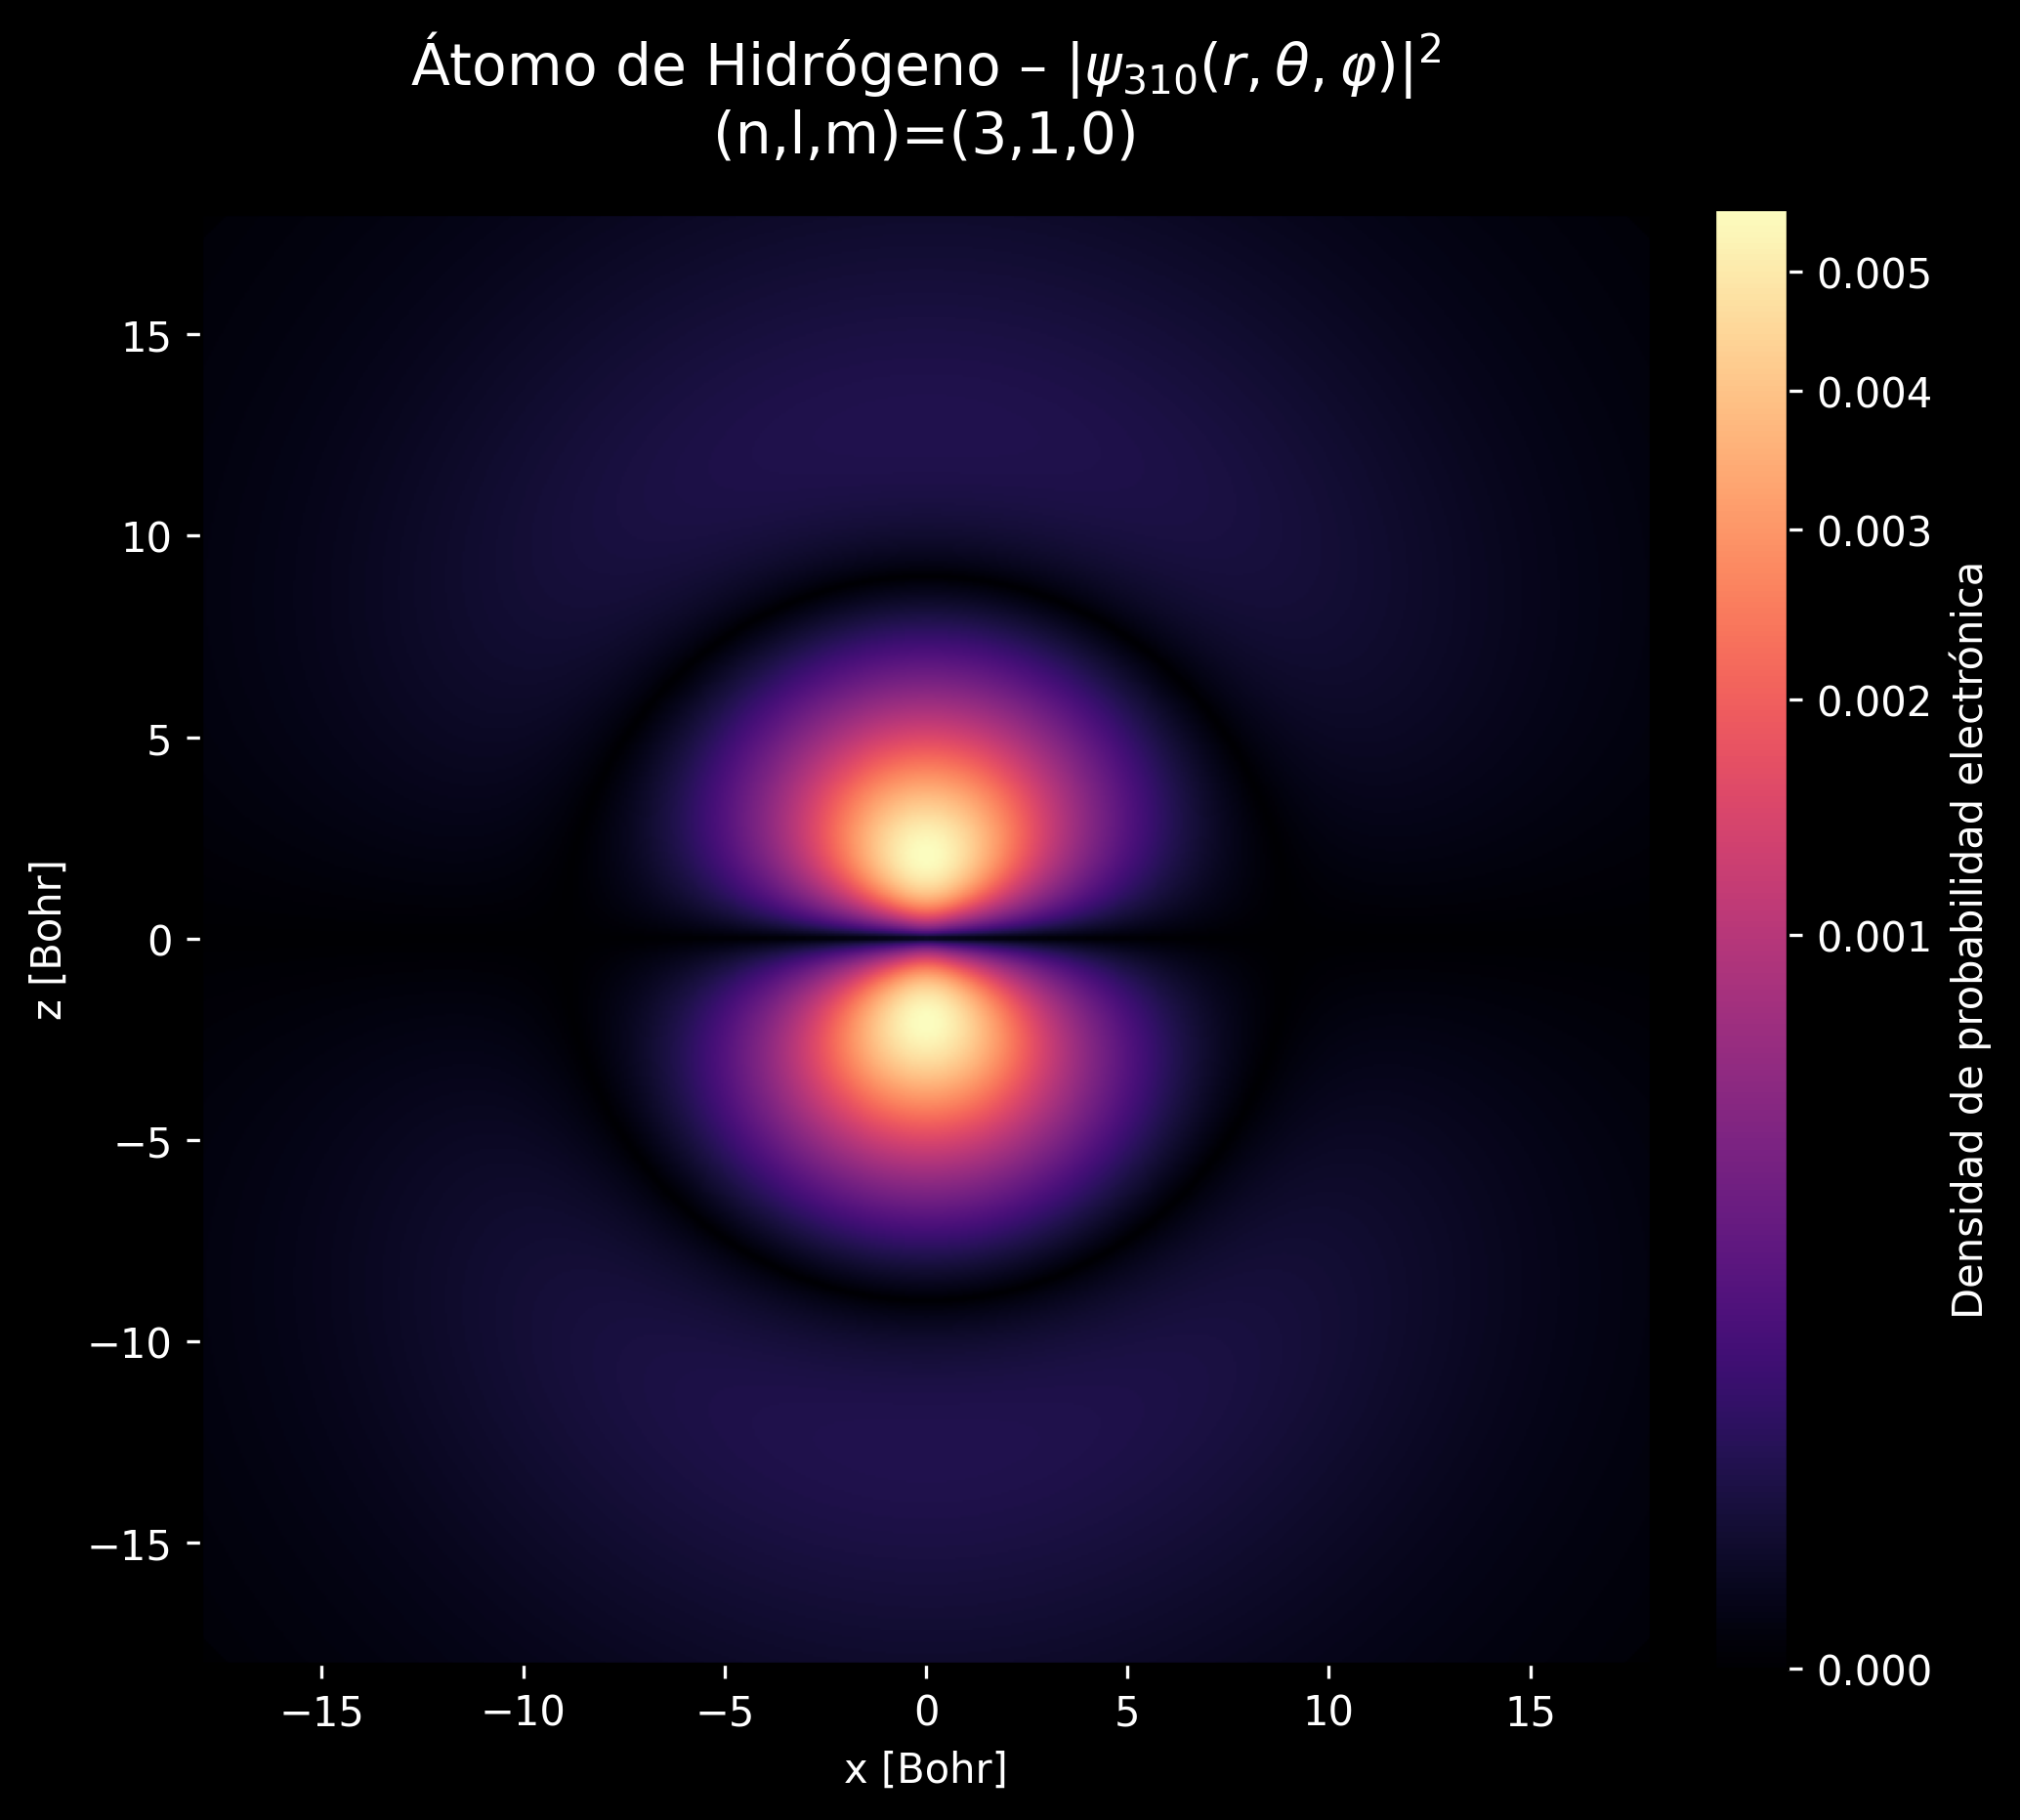
\includegraphics[width=\linewidth]{hydrogen_310.png}
\end{center}
  
}


\headerbox{SCF}{name=scf,column=2,below=intro,span=1}{

\resizebox{\linewidth}{!}{ 
\begin{tikzpicture}[node distance=1.4cm]

% Nodos
\node (start) [startstop] {Definir molécula: $\{R_A, Z_A, N\}$ en una base $\{\phi_\mu\}$};
\node (integrals) [process, below=of start] {Calcular integrales: $S_{\mu\nu}$, \(H_{\mu\nu}\), $(\mu\nu|\lambda\sigma)$};
\node (guess) [process, below=of integrals] {Iniciar matriz de densidad $P=0$};
\node (fock) [process, below=of guess] {Matriz de Fock: $F = H + G(P)$};
\node (transform) [process, below=of fock] {Ortogonalizar la base: $X^\dagger S X = I$};
\node (diag) [process, below=of transform] {Diagonalizar Fock en la nueva base: $F' = X^\dagger F X \Rightarrow C', \varepsilon$};
\node (update) [process, below=of diag] {Actualizar $C = X C'$ y nueva densidad $P_{\mu\nu} = 2\sum_i C_{\mu i}C_{\nu i}$};
\node (conv) [decision, below=of update, yshift=-0.2cm] {Convergencia?};
\node (end) [startstop, below=of conv, yshift=-0.2cm] {Terminar SCF};

% Flechas
\draw [arrow] (start) -- (integrals);
\draw [arrow] (integrals) -- (guess);
\draw [arrow] (guess) -- (fock);
\draw [arrow] (fock) -- (transform);
\draw [arrow] (transform) -- (diag);
\draw [arrow] (diag) -- (update);
\draw [arrow] (update) -- (conv);
\draw [arrow] (conv) -- node[right]{Sí} (end);
\draw [arrow] (conv.west) -| ++(-3,0) |- node[above left]{No} (fock.west);

\end{tikzpicture}
}

}
% \headerbox{SCF}{name=scf,column=2,below=intro,span=1,bottomaligned=code1}{
% 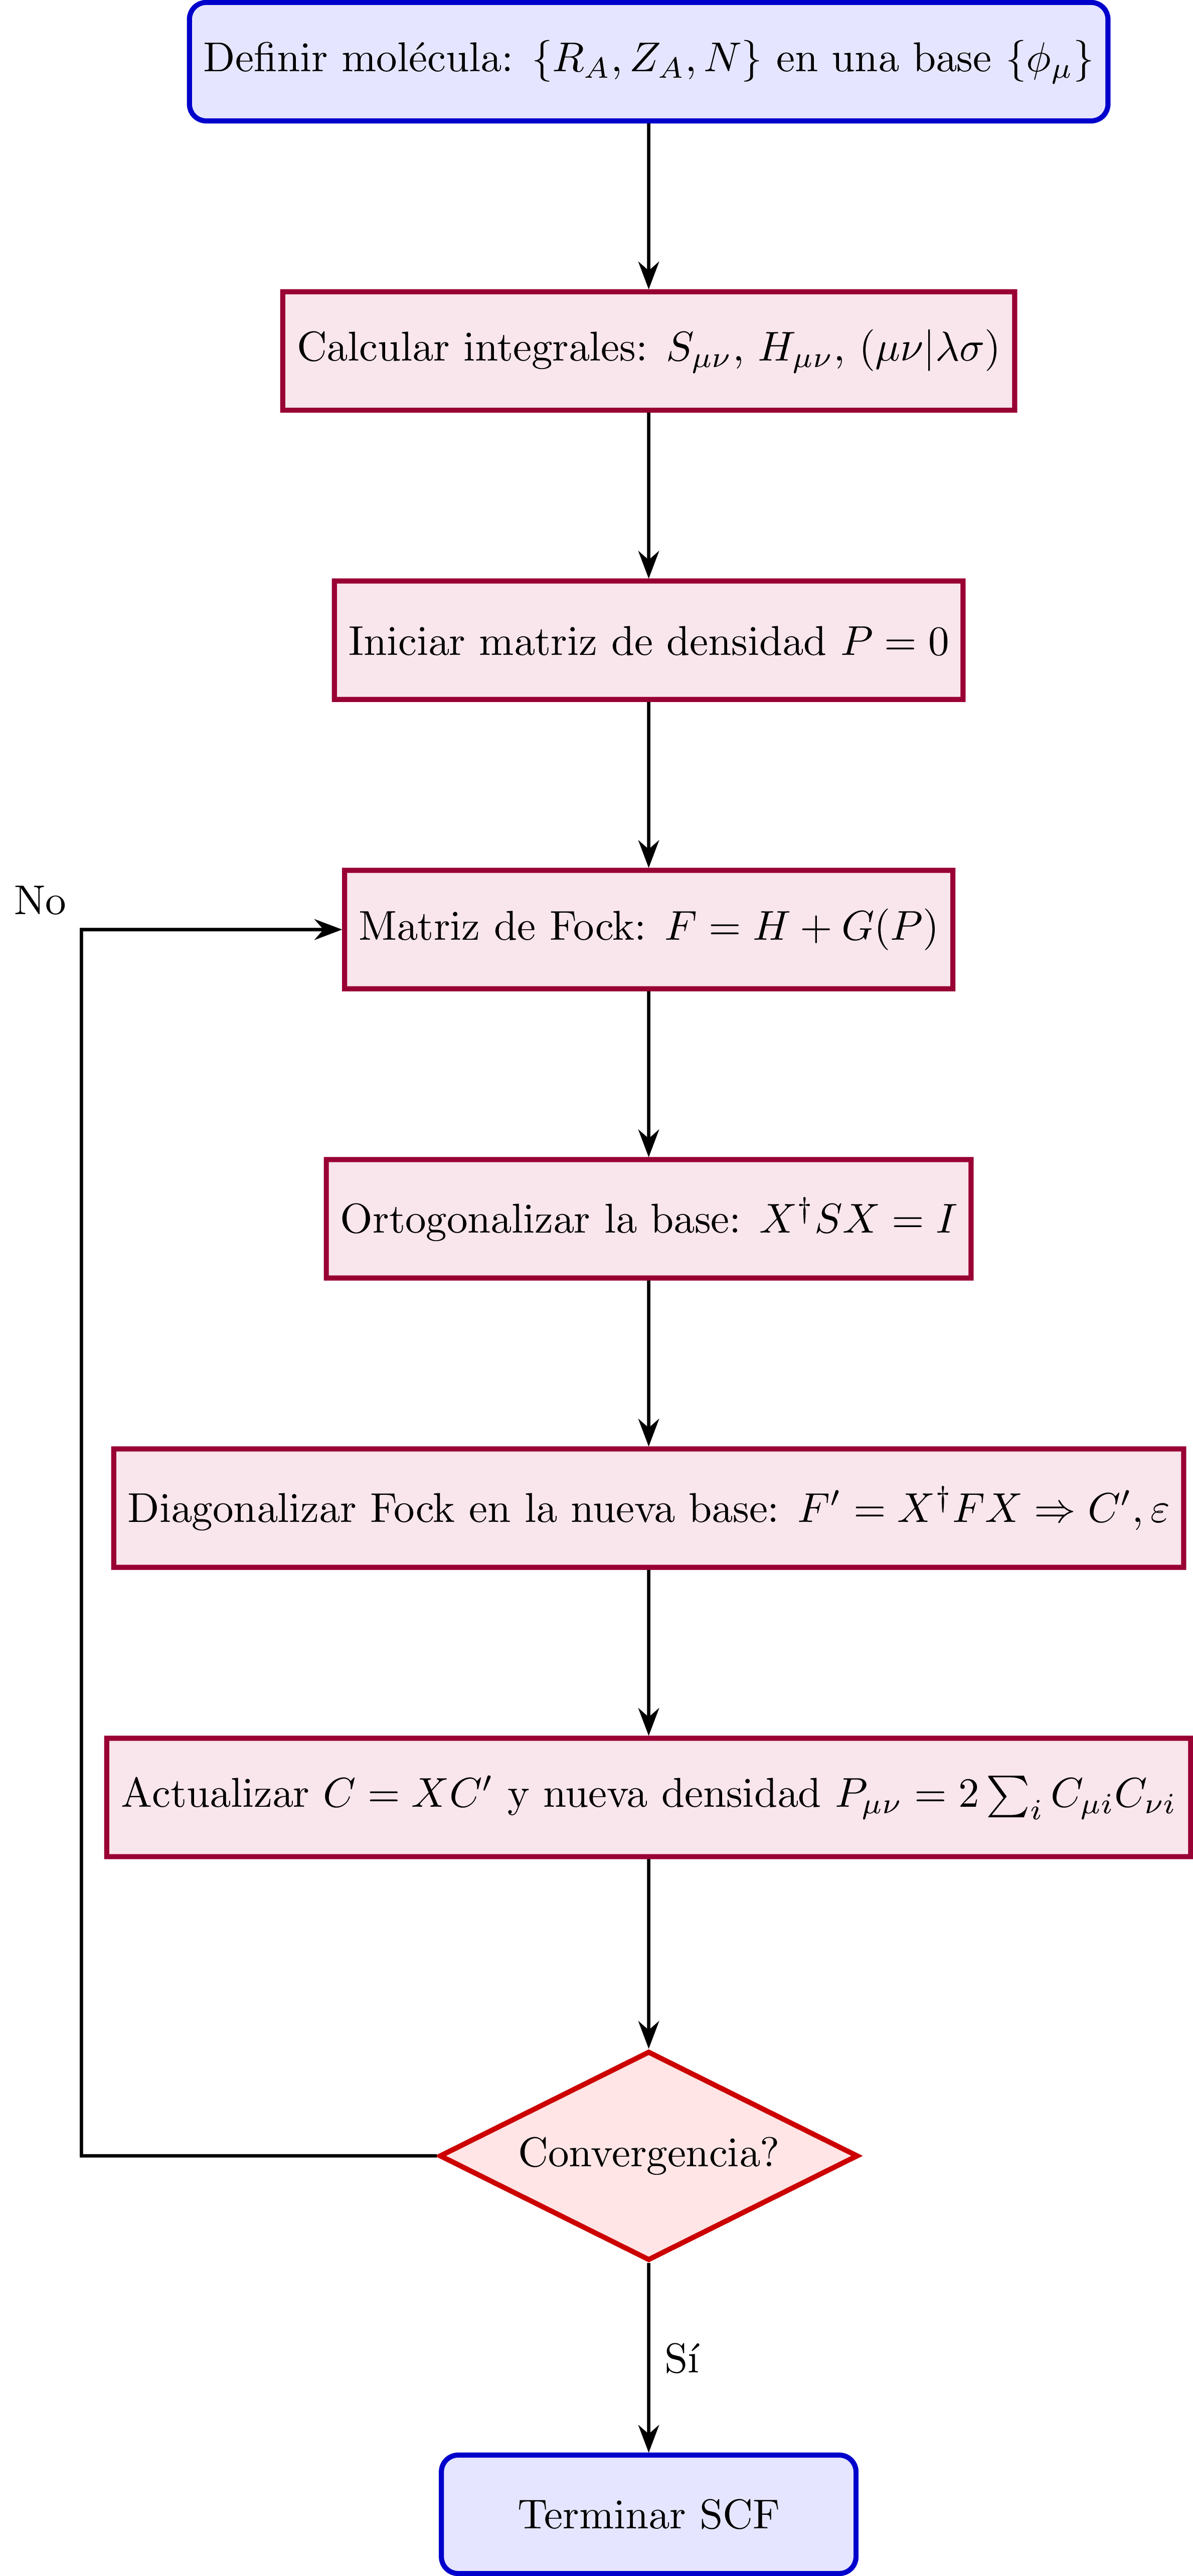
\includegraphics[width=\linewidth]{scf_diagram}
% }


%--------------------------------------------------
%	NUMEROV
%--------------------------------------------------


\headerbox{Numerov}{name=numerov,column=0,below=hf,span=1}{

El método de Numerov permite integrar ecuaciones diferenciales de segundo orden como la ecuación de Schrödinger adimensional:

\begin{equation}
\label{eq:2}
\pdv[2]{\Psi}{\xi} = -2\qty(\epsilon - \frac{\xi}{2})\Psi
\end{equation}

Formula de recurrencia de Numerov:

\begin{equation}
\label{eq:3}
\Psi_{n+1} = 
\frac{(12 - 10 f_n) \Psi_n - f_{n-1} \Psi_{n-1}}{f_{n+1}}
\end{equation}

\begin{center}
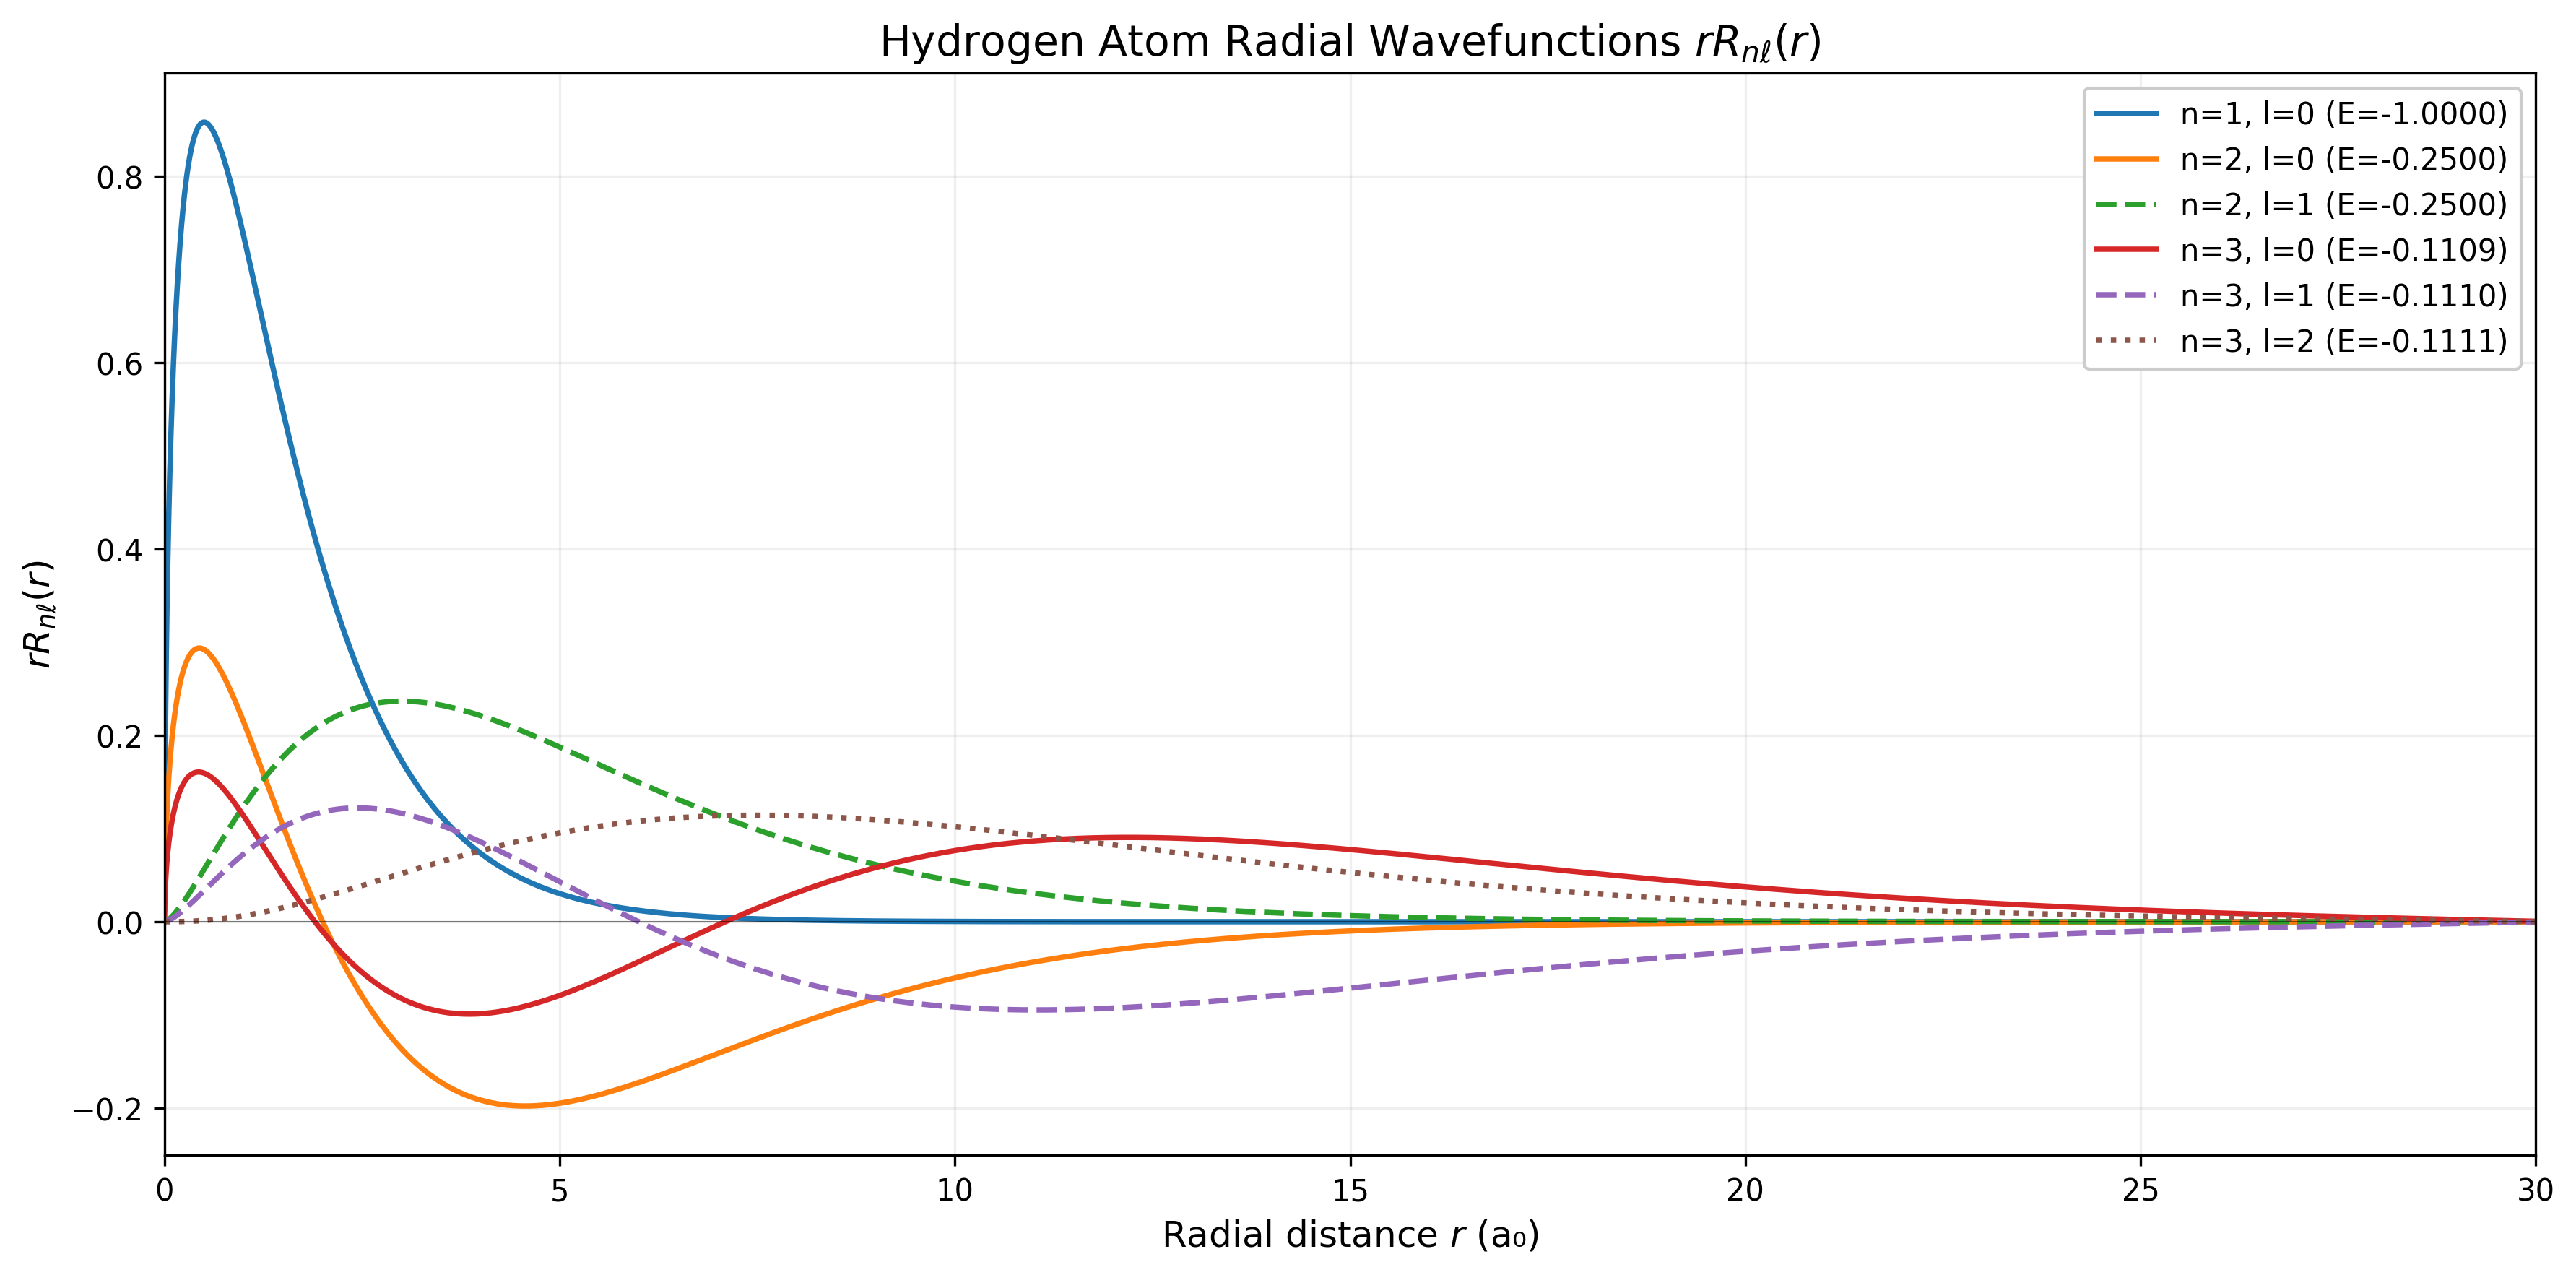
\includegraphics[width=\linewidth]{hydrogen.png}
\captionof{figure}{Funciones de onda radiales obtenidas con Numerov.}
\end{center}
  
}



\headerbox{Conclusiones}{name=conc,column=1,below=code1,span=2,bottomaligned=numerov}{
Comprender un método numérico desde su formulación hasta su implementación es una forma de investigación formativa.
El proyecto busca que el estudiante no solo use algoritmos, sino que piense como el físico que los concibió.
}

\headerbox{Repositorio}{name=qr,column=2,below=scf,span=1,bottomaligned=code1}{
\begin{center}
\qrcode[height=3cm]{https://recore799.github.io/schrodinger1d/}
\end{center}

}



\end{poster}
\end{document}
